%$LuaLaTeX -*- coding: utf-8 ; mode: latex; TeX-engine: luatex; -*-
\documentclass[a4paper]{book}

\usepackage[english, bidi=basic-r, layout=counters]{babel}

\babelprovide[import=ar, main]{arabic}

\babelfont{rm}
          [ItalicFont=FreeSerif, Numbers=Arabic]
          {FreeSerif}
\babelfont[english]{rm}{FreeSerif} % We need some italics

\usepackage{microtype}
\usepackage{graphicx}
\usepackage{color}
\usepackage{hyperref}
\usepackage{multicol}
\usepackage{booktabs}

\title{كهرباء} \author{From Wikipedia}

% Fix some bad kerns inserted by the font loader. I don't know where
% the bug is and why the following workaroud fixes it. It just forces
% a dir node as the second node in the par. Note it doesn't take hboxes
% into account, yet (no local_par = 9 node at the beginning). It seems
% the font loader will be fixed soon.

\directlua{

function fixkerns (head)
  if head and head.id == 9 then
    snd = head.next
    if snd and not (snd.id == node.id'dir') then
      local d = node.new(node.id'dir')
      d.dir = head.dir
      head = node.insert_after(head, head, d)
    end
  end
  return head
end

where = luatexbase.priority_in_callback('pre_linebreak_filter',
        'luaotfload.node_processor')

luatexbase.add_to_callback("pre_linebreak_filter", fixkerns, "fixkerns", where)
% luatexbase.add_to_callback("hpack_filter", fixkerns, "fixkerns", where)
}

\begin{document}

\frontmatter

\maketitle

\tableofcontents

\chapter{مقدمة}

الكهرباء اسم يضم مجموعة متنوعة من الظواهر الناتجة عن وجود شحنة
كهربائية وتدفقها. وتضم هذه الظواهر البرق والكهرباء الساكنة. ولكنها
تحتوي على مفاهيم أقل شيوعًا مثل المجال الكهرومغناطيسي والحث
الكهرومغناطيسي.

أما في الاستخدام العام، فمن المناسب استخدام كلمة «كهرباء» للإشارة إلى
عدد من التأثيرات الفيزيائية. ولكن في الاستخدام العلمي، يعد المصطلح
غامضًا. كما أن هذه المفاهيم المتعلقة به يُفضل تعريفها وفقًا لمصطلحات أكثر
دقة كما يلي:

\begin{description}
\item[الشحنة الكهربائية] هي خاصية لبعض الجسيمات دون الذرية تحدد
التفاعلات الكهرومغناطيسية الخاصة بها. فالمادة المشحونة كهربائيًا تتأثر
بالمجالات الكهرومغناطيسية وتنتجها.
\item[التيار الكهربائي] هو تحرك أو تدفق الجسيمات المشحونة كهربائيًا،
ويُقاس عادةً بالأمبير.
\item[المجال الكهربائي] هو تأثير تنتجه شحنة كهربائية في غيرها من
الشحنات الموجودة بالقرب منها.
\item[الجهد الكهربائي] قدرة المجال الكهربائي على الشغل، ويُقاس عادةً
بوحدة الفولت.
\item[الكهرومغناطيسية] هي التفاعل الأساسي الذي يحدث بين المجال
المغناطيسي ووجود الشحنة الكهربائية وحركتها.
\end{description}

خضعت الظواهر الكهربائية للدراسة منذ القِدم، إلا أن علم الكهرباء لم يشهد
أي تقدم حتى القرنين السابع عشر والثامن عشر. ومع ذلك فقد ظلت التطبيقات
العملية المتعلقة بالكهرباء قليلة العدد، ولم يتمكن المهندسون من تطبيق
علم الكهرباء في الحقل الصناعي والاستخدامات السكنية إلا في أواخر القرن
التاسع عشر. وقد أدى التقدم السريع في تكنولوجيا الكهرباء في ذلك الوقت
إلى إحداث تغييرات في المجال الصناعي وفي المجتمع أيضًا. كما أن
الاستعمالات المتعددة والمذهلة للكهرباء كمصدر من مصادر الطاقة أظهر
إمكانية استخدامها في عدد كبير من التطبيقات مثل المواصلات والتدفئة
والإضاءة والاتصالات والحساب. فأساس المجتمع الصناعي الحديث يعتمد على
استخدام الطاقة الكهربائية، ويمكن التكهن بأن الاعتماد على الطاقة
الكهربائية سيستمر في المستقبل.

\bigskip

\foreignlanguage*{english}{Below, in red, a couple of words
incorrectly rendered by default in the corrent font. It seems a bug in
the font loader, and a workaround is used in this document (see the
source).}

\mainmatter

\chapter{نظرة عامة}

\section{وجه التسمية}

الكهرباء لفظ فارسي مركب من کاه أي القش ومن رُبَای أي الجاذب، ومعناها
جميعا جاذب القش؛ والمراد بكلمة کهربا في الفارسية هو الكهرمان المسمى
بالعربية العنبر الأشهب، أما المقصود من كلمة الكهرباء في العربية فهو
"جاذبية الكهرمان" والتي كانت تسمى بالعربية خاصية الكهرباء فحذفوا كلمة
الخاصية واكتفوا بلفظ الكهرباء. وبذلك تحول من الفارسية إلى العربية من
معنى الفاعل (الجاذب) إلى معنى الفاعلية (الجاذبية).

الكهرمان اسمه باليونانية الإيلقطرون[3] (معرب ἤλεκτρον إيلكترون أي ذو
البريق، ومنه الإلكترون عند الفيزيائيين، وعليه تسمية الكهرباء في
الفارسية برق)، واشتق منه اسم فاعليتيه فسمي إلكترسمس (ηλεκτρ‌ισμός)
للدلالة على الكهرباء. أما باللاتينية فالكلمة للكهرباء هي إيلكترستاس
(ēlectricitās)، وهي مشتقة من إيلكتركس (ēlectricus) أي شبيه الكهرمان.

\section{تاريخ}

قبل معرفة الكهرباء بفترة طويلة، كان الناس على دراية بالصدمات التي
يحدثها سمك الرعاش، وقد أشارت النصوص التي تركها قدماء المصريين، والتي
يرجع تاريخها إلى سنة 2750 قبل الميلاد، إلى هذه الأسماك باسم "صاعقة
النيل"، كما وصفوها بأنها حامية جميع الأسماك الأخرى. وبعد حوالي ألف
عام، أشار إليها أيضًا الإغريق والرومان وعلماء الطبيعة والأطباء
المسلمون.[4] ولقد أكد الكتّاب القدامى، مثل بليني الأكبر وسكريبونيس
لارجوس على الإحساس بالتنميل الناتج عن الصدمات الكهربائية التي يحدثها
سمك السلّور الصاعق وأنقليس الرعاد الكهربائي. كما اكتشف هؤلاء الكتّاب أن
هذه الصدمات يمكن أن تنتقل عبر الأجسام الموصلة.[5] وبجميع الأحوال، ينسب
أقدم وأقرب أسلوب لاكتشاف ماهية البرق والكهرباء الصادرة عن أي مصدر آخر
إلى العرب الذين أطلقوا كلمة "برق" العربية على الشعاع الكهربائي قبل
القرن الخامس عشر. وقد كان معروفًا في الثقافات القديمة للدول المطلة على
البحر الأبيض المتوسط أن هناك أجسامًا معينة مثل قضبان الكهرمان، يمكن
حَكِّها بفرو قطة فتجذب الأجسام الخفيفة مثل الريش. وقد قام العالم
والفيلسوف الإغريقي، طاليس الملطي، حوالي عام 600 قبل الميلاد بتسجيل
مجموعة من الملاحظات تتعلق بالكهرباء الساكنة. وبعد هذه الملاحظات، توصل
إلى أن الاحتكاك يحول الكهرمان إلى مادة مغناطيسية. وعلى عكس ذلك، لا
تحتاج المعادن، مثل الماغنتيت المعروف باسم أكسيد الحديد الأسود، إلى
عملية الاحتكاك حتى تكتسب صفة المغناطيسية.[6] إلا أن طاليس كان مخطئًا في
اعتقاده بأن سبب الانجذاب هو التأثير المغناطيسي، فقد أثبتت الأبحاث
العلمية فيما بعد وجود علاقة بين المغناطيسية والكهرباء. ووفقًا لإحدى
النظريات المثيرة للجدل، فقد عرف البارثيون، إحدى شعوب بلاد فارس، الطلاء
الكهربائي وفقًا لما أفادت المعلومات التي تحصلت من اكتشاف بطارية بغداد
عام 1936. وعلى الرغم من أن هذه البطارية تشبه الخلية الجلفانية، فإنه من
غير المؤكد ما إذا كانت ذات طبيعة كهربية أم لا.

\begin{figure}
\centering
  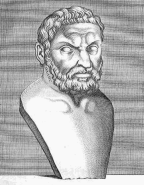
\includegraphics{Thales.png}
  \caption{طاليس، أول باحث في الكهرباء.}
\end{figure}

ظلت الكهرباء لا تعني أكثر من مجرد فضول فكري لآلاف السنين حتى عام
1600. ففي ذلك العام، أجرى الطبيب الإنجليزي ويليام جيلبرت دراسة دقيقة
حول الكهرباء والمغناطيسية، وفرّق فيها بين تأثير حجر المغناطيس والكهرباء
الساكنة التي تنتج عن احتكاك مادة الكهرمان.[6] وابتكر كلمة «electricus»
وهي باللغة اللاتينية الجديدة («من الكهرمان» أو «شبيه الكهرمان»،
ومأخوذة من «ήλεκτρον» أي «إلكترون»، وهي المرادف اليوناني لكلمة
«كهرمان») للإشارة إلى خاصية جذب الأجسام الصغيرة بعد حكها. [7] أدى هذا
الارتباط إلى إبراز الكلمتين «Electric» و«Electricity» اللتين ظهرتا
لأول مرة في كتاب توماس براون «الأخطاء الشائعة» (باللاتينية:
Pseudodoxia Epidemica) الذي صدر عام 1646.

 قد قدم أوتو فون جيريك وروبرت بويل وستيفن جراي وسي إف ديو فاي المزيد من
الأعمال. وأجرى بنيامين فرانكلين في القرن الثامن عشر أبحاثًا شاملة بشأن
الكهرباء، حتى أنه اضطر إلى بيع ممتلكاته لتمويل أبحاثه. وقيل أنه في شهر
حزيران/يونيو من سنة 1752، قام بربط مفتاح معدني أسفل خيط طائرة ورقية
رطب وأطلق الطائرة في سماء تنذر بهبوب عاصفة. ثم لاحظ مجموعة متلاحقة من
الشرارات تخرج من المفتاح إلى ظهر يده، الأمر الذي \textcolor{red}{برهن}
على أن البرق ذو طبيعة كهربائية بالفعل. [9] نشر لودجي جالفاني عام 1791
اكتشافه الخاص بالكهرباء الحيوية الذي أظهر أن الكهرباء هي الوسيط الذي
تقوم من خلاله الخلايا العصبية بنقل \textcolor{red}{الإشارات} إلى
العضلات.

\subsection{التيار الكهربائي}

\begin{multicols}{3}
  تُعرف حركة الشحنة الكهربائية باسم التيار الكهربائي الذي تقاس شدته
  عادةً بوحدة الأمبير. ويتكون التيار الكهربائي من أية جسيمات مشحونة
  ومتحركة. وتعد الإلكترونات الأكثر شيوعًا بين هذه الجسيمات، ولكن أي
  شحنة متحركة يمكنها أن تكون تيارًا. ووفقًا لما هو متعارف عليه، فإن
  التيار الموجب يُعَرّف بأنه التيار المتدفق في الاتجاه نفسه الذي تتدفق
  فيه أية شحنة موجبة يحملها؛ أو أنه التيار المتدفق من أقصى طرف موجب في
  الدائرة الكهربائية إلى أقصى طرف سالب. ويُطلق على هذا النوع من
  التيارات اسم التيار الاصطلاحي. وبالتالي، تعد حركة الإلكترونات
  السالبة حول الدائرة الكهربائية ـ وهي أحد أشهر أشكال التيار الكهربائي
  ـ موجبة في الاتجاه المقابل لاتجاه الإلكترونات.[22] ومع ذلك، فإنه
  وفقًا للظروف المحيطة يمكن أن يتكون التيار الكهربائي من تدفق الجسيمات
  المشحونة (الجسيم المشحون) في أيٍّ من الاتجاهين أو حتى في كلا الاتجاهين
  في وقت واحد. ويشيع استخدام المصطلحين السالب والموجب لتبسيط هذه
  الحالة.

  علاوةً على ذلك، يُطلق على العملية التي يمر فيها التيار الكهربائي خلال
  أحد المواد "التوصيل الكهربائي". وتختلف طبيعة التوصيل الكهربائي عن
  طبيعة الجسيمات المشحونة والمادة التي يمر من خلالها. ومن أمثلة
  التيارات الكهربائية: التوصيل الفلزي الذي تتدفق فيه الإلكترونات خلال
  موصل مثل الفلز. بالإضافة إلى ذلك، هناك التحليل الكهربائي الذي تتدفق
  فيه الأيونات (وهي عبارة عن ذرات مشحونة) خلال السوائل. في حين تتحرك
  الجسيمات نفسها ببطء تام، ليصل متوسط سرعة الانسياق أحيانًا إلى أجزاء
  من المليمتر في الثانية،[21] فإن المجال الكهربائي الذي تتدفق فيه هذه
  الجسيمات ينتشر في حد ذاته بسرعة مقاربة لسرعة الضوء، مما يسمح
  للإشارات الكهربائية بالمرور بسرعة خلال الأسلاك.[23] يؤدي التيار
  الكهربائي إلى حدوث عدة تأثيرات ملحوظة ـ كانت تعتبر في الماضي الوسيلة
  التي يدرك بها الأفراد وجود تيار كهربائي. وقد اكتشف ويليام نيكلسون
  وأنطوني كارلايل عام 1800 أن بإمكان التيار الكهربائي تحليل الماء من
  بطارية فولتية، وتُعرف هذه العملية الآن باسم التحليل الكهربائي. وقام
  مايكل فاراداي بعمل دراسات موسعة في اكتشاف نيكلسون وكارلايل بشكل كبير
  عام 1833.[24] ويسبب التيار المار من خلال مقاومة نوعًا من التدفئة في
  المكان المحيط، وهو تأثير كان جيمس بريسكوت قد بحثه حسابيًا عام
  1840. ومن أهم الاكتشافات الخاصة بالتيار الكهربائي كان ما توصل إليه
  هانز كريستيان أورستد بمحض الصدفة عام 1820 عندما كان يحضر إحدى
  محاضراته. حيث وجد أن التيار الكهربائي في أحد الأسلاك يشوش حركة إبرة
  البوصلة المغناطيسية،[25] كما اكتشف الكهرومغناطيسية، وهي عبارة عن
  تفاعل أساسي يحدث بين الكهرباء والمغناطيسات.
\end{multicols}

\subsection{جدول التوزيع الإلكتروني}

\foreignlanguage*{english}{Also from Wikipedia. These examples show
the column order and some directions must be still sorted out. See the
source for the workaroud used here. Furthermore, the way “New
Caledonia” is split looks wrong (but actually “correct”).}

\let\ortabular\tabular
\def\tabular{\mathdir\pagedir\ortabular}

\begingroup

\addfontfeatures{Numbers=ArabicOff}

\begin{center}
\begin{tabular}{lllllllll}
\toprule
\multicolumn{1}{c}{الرقم} & العنصر & 1 & 2 & 3 & 4 & 5 & 6 & 7\\
\cmidrule(r){1-2}\cmidrule(r){3-9}
1 & هيدروجين & 1\\
2 & هيليوم & 2\\
37 & روبيديوم & 2 & 8 & 18 & 8 & 1\\
38 & سترانشيوم & 2 & 8 & 18 & 8 & 2\\
39 & إيتيريوم & 2 & 8 & 18 & 9 & 2\\
40 & زركونيوم & 2 & 8 & 18 & 10 & 2\\
41 & نيوبيوم & 2 & 8 & 18 & 12 & 1\\
42 & موليبيدنيوم & 2 & 8 & 18 & 13 & 1\\
\bottomrule
\end{tabular}
\end{center}

\endgroup

\begin{center}
\begin{tabular}{lp{8cm}}
  \toprule
  الشعاب المرجانية
  & شعب حلقي • Cay • Fringing reef • Microatoll •
    سمك المرجان • \foreignlanguage{english}{\textit{The Structure and
    Distribution of Coral Reefs}}\\[1ex]
  مناطق الشعاب  المرجانية
  & Deep water coral • اندروس وجزر البهاما • الحاجز المرجاني لبليز •
    جزر بحر المرجان • مثلث الشعاب • الحيد المرجاني العظيم • جزر المالديف •
    Mesoamerican Barrier Reef System • New Caledonia Barrier Reef • Pulley
    Ridge • جزر راجا أمبات • البحر الأحمر • Southeast Asian coral reefs\\
  \bottomrule
\end{tabular}
\end{center}

\end{document}
